%
% resultat.tex 
%
% 
%
% !TEX root = ../../buch.tex
% !TEX encoding = UTF-8
%

\section{Resultat\label{antennen:resultat}}

Lösung war ja ein Kreis nun beschreiebn wir 3eck mit radius

\subsection{Parametrisierung Dreieck\label{antennen:param3eck}}

\begin{figure}[htbp]
	\centering
	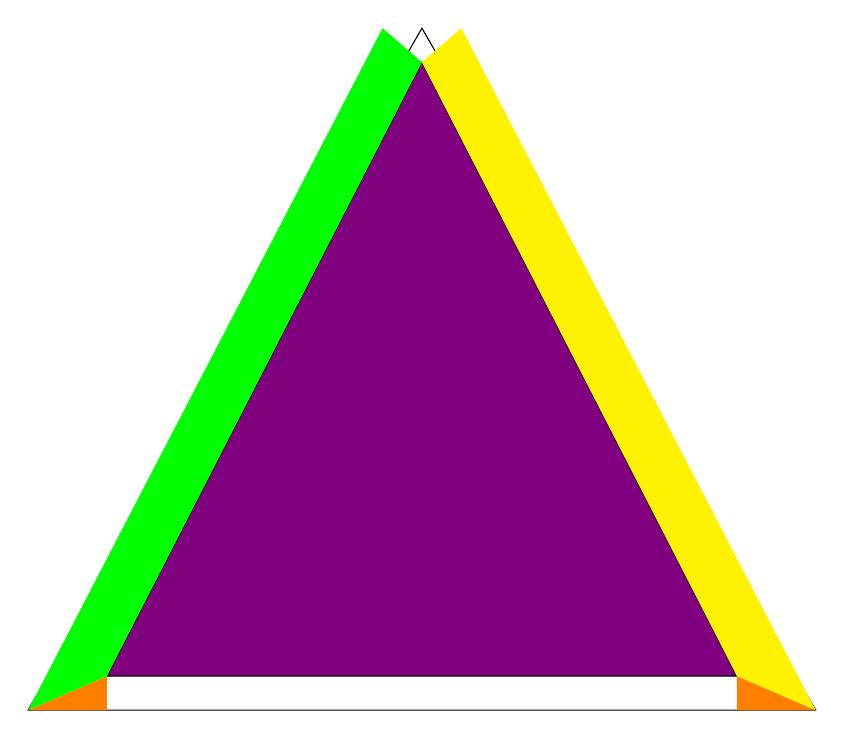
\begin{tikzpicture}
		% Define the length of the sides of the triangles
		\def\sidelength{10}
		
		% Calculate the height of the equilateral triangle
		\pgfmathsetmacro{\triangleheight}{sqrt(3)/2*\sidelength}
		
		% Draw the large outer triangle (white background)
		\draw[fill=white] (0,0) -- (\sidelength,0) -- (0.5*\sidelength, \triangleheight) -- cycle;
		
		% Draw the main central triangle (purple)
		\draw[fill=blue!50!red] (0.1*\sidelength, 0.05*\triangleheight) -- (0.9*\sidelength, 0.05*\triangleheight) -- (0.5*\sidelength, 0.95*\triangleheight) -- cycle;
		
		% Draw the colored segments at each edge
		% Bottom edge segments
		\fill[orange] (0,0) -- (0.1*\sidelength,0) -- (0.1*\sidelength, 0.05*\triangleheight) -- cycle;
		\fill[orange] (\sidelength,0) -- (0.9*\sidelength,0) -- (0.9*\sidelength, 0.05*\triangleheight) -- cycle;
		
		% Left edge segments
		\fill[green] (0,0) -- (0.1*\sidelength, 0.05*\triangleheight) -- (0.5*\sidelength, 0.95*\triangleheight) -- (0.45*\sidelength, \triangleheight) -- cycle;
		
		% Right edge segments
		\fill[yellow] (\sidelength,0) -- (0.9*\sidelength, 0.05*\triangleheight) -- (0.5*\sidelength, 0.95*\triangleheight) -- (0.55*\sidelength, \triangleheight) -- cycle;
		
	\end{tikzpicture}
	\caption{Stylized triangle plot created with TikZ.}
	\label{antennen:tikzparam3eck}
\end{figure}

dasdasd \ref{antennen:tikzparam3eck} dasda